\section{Robotic Interaction Model}
\label{sec:interactivemodel}
% \begin{figure*}
\centering
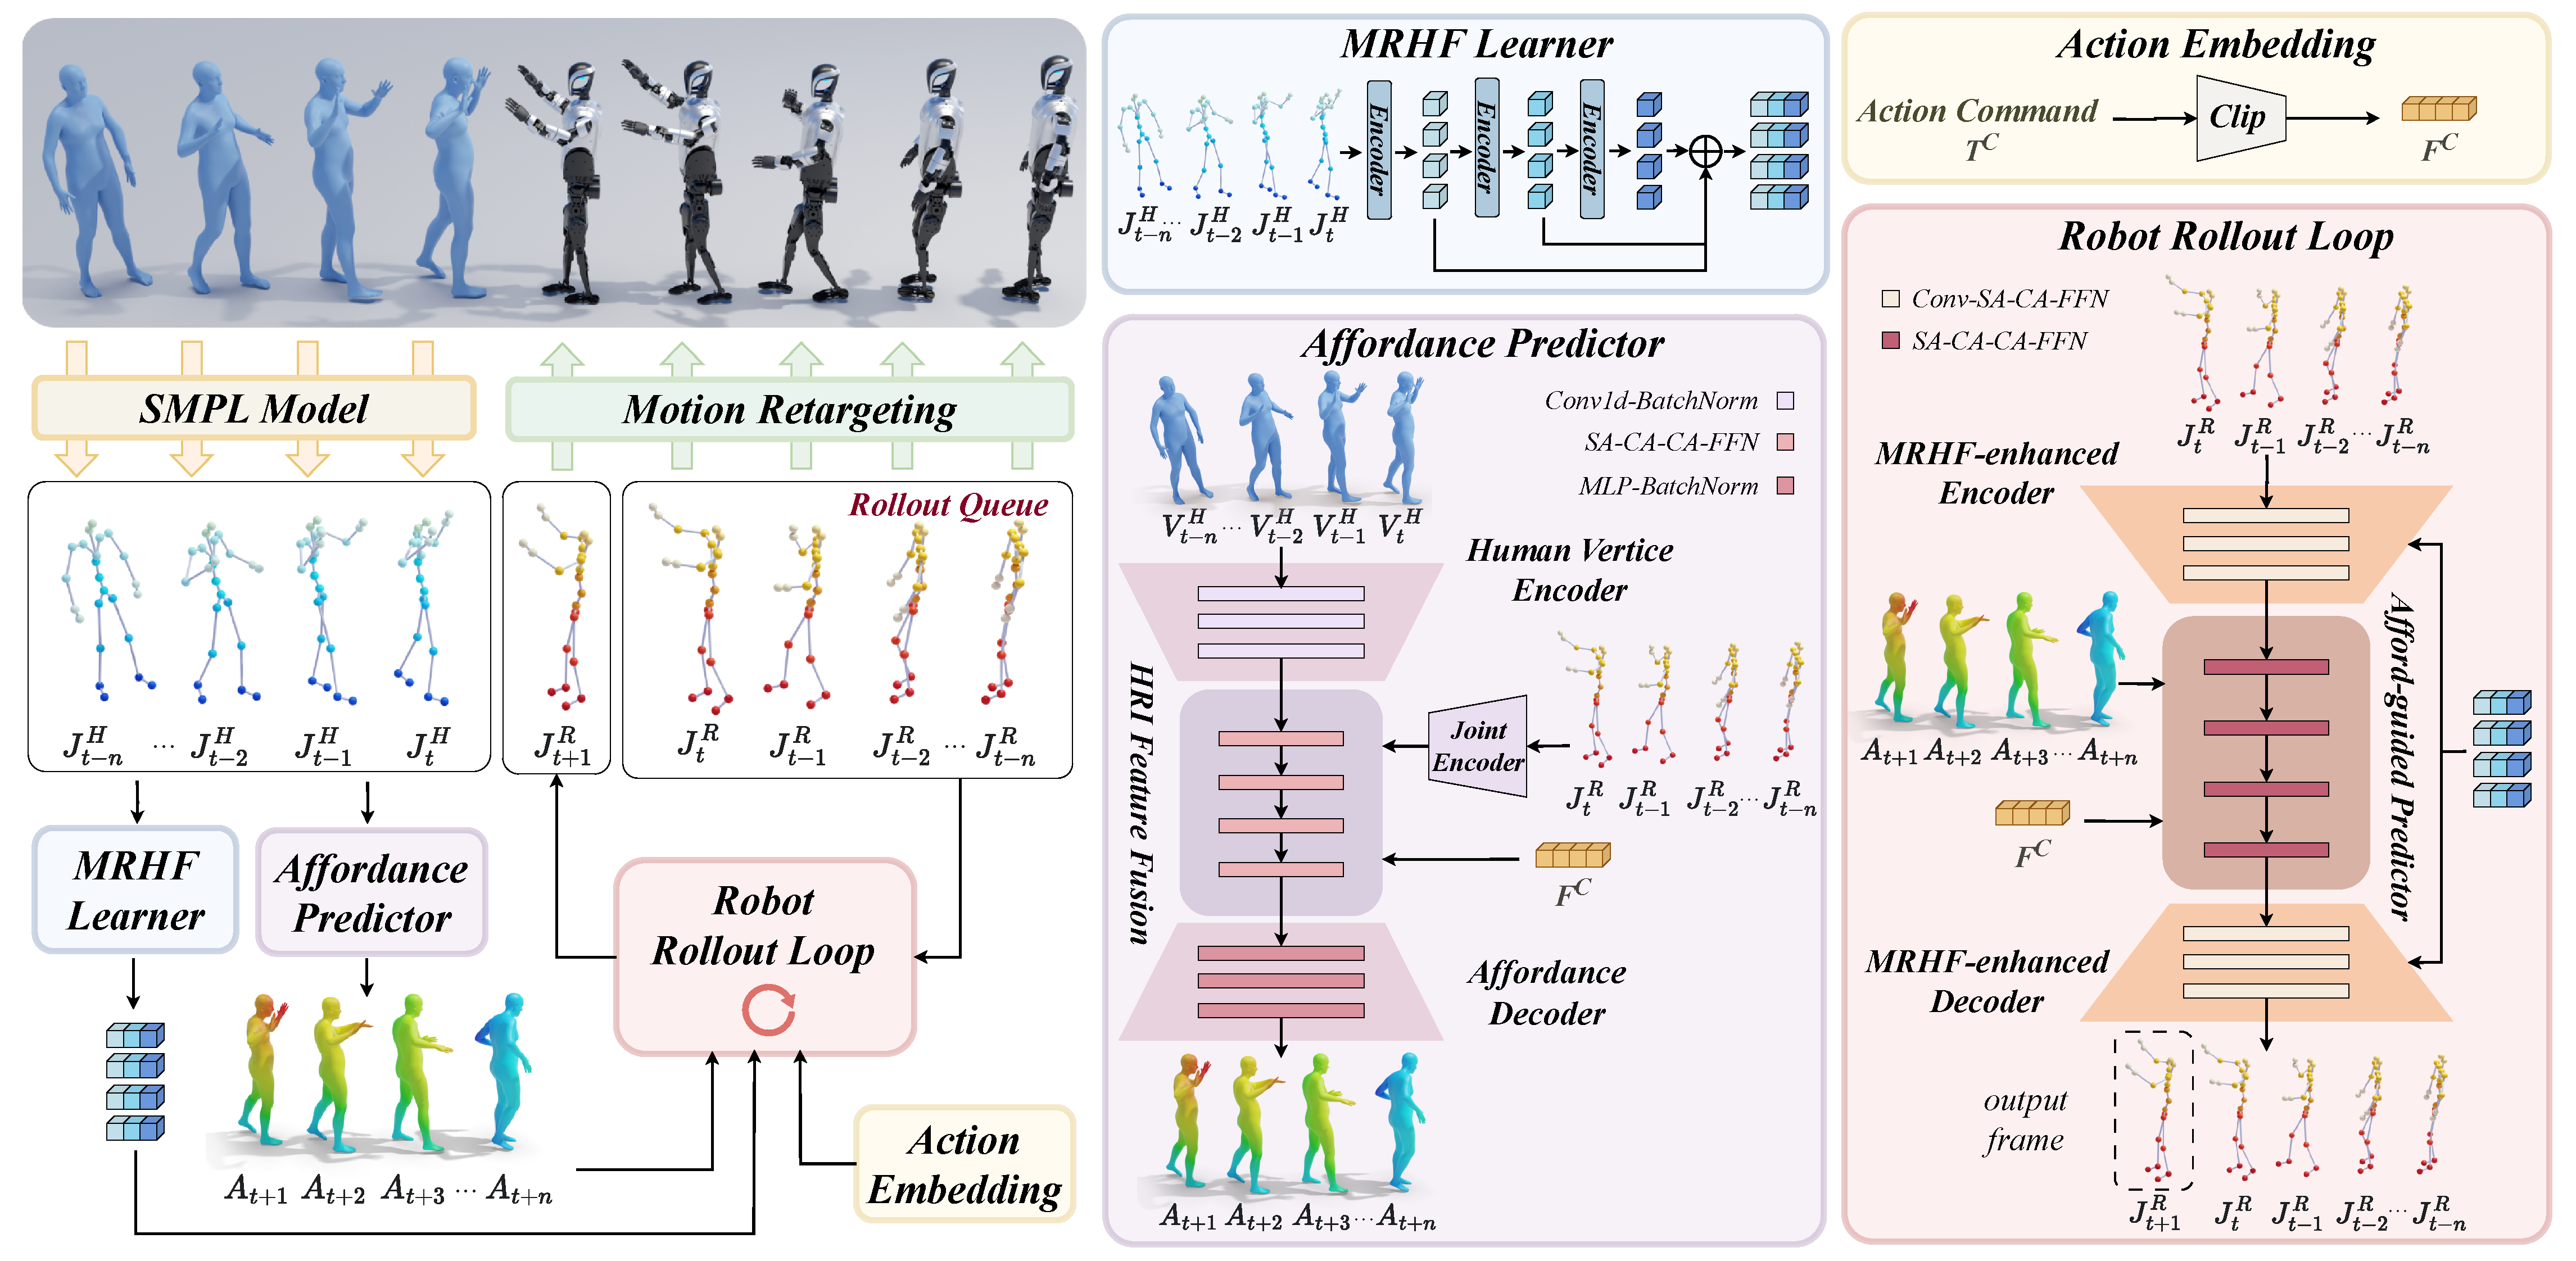
\includegraphics[width=1\linewidth]{images/intermodel-mainv5.pdf}
\vspace{-20pt}
\caption{Overall pipeline of our Robotic Interaction Model. The model ingests text action commands, historical robot joints, observed human joints and SMPL mesh vertices, and processes them through four tightly coupled modules. The Affordance Predictor explicitly estimates dense end-effector–vertex spatial fields to enable dexterous, socially-appropriate contact reasoning; the Multi-Resolution Human Feature (MRHF) Learner fuses hierarchical temporal cues to boost situational awareness; the Robot Rollout Loop leverages these affordance and human features to iteratively generate coherent, context-adaptive joint trajectories for real-time responsiveness; and finally, the Motion Retargeting module maps each predicted skeleton frame to robot-specific angle axis.}
\label{fig:interactiveModel}
\vspace{-10pt}
\end{figure*}

Real-time, context-aware motion generation remains a persistent challenge for human-robot interaction, especially in dynamic and contact-rich scenarios.
Existing approaches~\cite{wang2021multi,xu2024regennet,mueller2024massively} for interactive robot motion generation often fail to adequately address real-time responsiveness and realistic interaction dynamics. To address these challenges, we propose a novel Robotic Interaction Model capable of generating coherent and timely interactive motion sequences for humanoid robot with three main technical advances:

%\begin{itemize}
\noindent\textbf{1) Affordance Predictor} precisely captures fine-grained spatial and geometric relationships between robot end-effectors and the human body, which is crucial for guiding the generation of precise and socially-appropriate interactive actions.
\noindent \textbf{2) Multi-Resolution Human Feature (MRHF) Learner} integrates human behavioral features at multiple temporal scales, improving the understanding of human intentions.
\noindent \textbf{3) Robot Rollout Loop} enables real-time, coherent, and context-adaptive robot motion, ensuring both responsiveness and long-term stability. It provides a solid guarantee for smooth and realistic interactive experience of the system.
%\end{itemize}


\subsection{Model Input and Output}
Our model generates humanoid robot motions in an online fashion by conditioning on both human behavior and robot history. As shown in Fig.~\ref{fig:interactiveModel}, the model takes three inputs at each timestep.
\noindent\textbf{Textual Command ($T^C$)} is a user-specified action prompt such as \textit{``High-five''} or \textit{``Handshake''}, representing the intended interaction type. Our Action Embedding module uses a pre-trained CLIP~\cite{radford2021learning} text encoder to map it to a visual-aware feature $F^C$, which is then fused with motion features in downstream modules to guide context-aware motion generation.
\noindent\textbf{Historical Robot Motion ($J^{R}_{t-n\sim t}$)} is a sequence of past robot joint skeletons, stored in a rollout queue from timestep $t - n$ to $t$. \noindent\textbf{Human Motion Observation} includes human joint skeletons ($J^{H}_{t-n\sim t}$) and SMPL mesh vertices ($V^{H}_{t-n\sim t}$). Both are obtained by applying the SMPL model to the pose parameters \( P^{H}_{t-n\sim t} \) and translation parameters \( T^{H}_{t-n\sim t} \) from the motion capture mentioned in Section~\ref{sec:mocap}. 


The model outputs a future sequence of predicted robot skeletons $J^R_{t+1 \sim t+k}$. We then employ a \textbf{receding horizon strategy}: only the immediate next frame $J^R_{t+1}$ is executed, while the rest of the sequence is discarded. This approach is crucial for balancing long-term motion coherence with real-time responsiveness. Predicting a multi-frame sequence ensures that the generated motion is smooth and natural, guided by sequence-level supervision. Conversely, executing only the first frame enables the robot to immediately adapt to dynamic human behavior by re-planning at every timestep. This continuous cycle not only guarantees high responsiveness but also enhances robustness by mitigating the accumulation of prediction errors.

% The model outputs a future sequence of predicted robot skeletons $J^{R}_{t+1\sim t+k}$ for the consistency of predicted robot motion. However, \textbf{only the immediate next frame} $J^{R}_{t+1}$ is executed by robot, and the rest of the sequence is discarded to guarantee online generation.




%The frame-by-frame rollout strategy enables real-time interactivity by:
%\textbf{Responsiveness}: Adapting quickly to unexpected human actions.
%\textbf{Robustness}: Avoiding error accumulation from long-term predictions (unlike offline methods~\cite{mueller2024massively,wang2021multi,xu2024regennet}).
%\textbf{Coherence}: Maintaining fluid motion by updating observations at each step.

%This approach mimics human-like adaptation, making the robot’s behavior dynamic and natural rather than rigid or pre-scripted.

%This \textbf{frame-by-frame rollout strategy} is essential to achieving real-time interactivity:
%\textbf{Responsiveness.} It allows the robot to adapt to rapid or unexpected changes in human behavior on-the-fly.
%\textbf{Robustness.} It avoids accumulation from long-term prediction errors, which is a common limitation of offline motion generation approaches~\cite{mueller2024massively,wang2021multi,xu2024regennet}.
%\textbf{Coherence.} By conditioning on updated observations at each step, the model maintains consistent and fluid behavior over time.
%This mechanism mirrors how humans naturally adjust their actions during interaction—based on continuous perceptual feedback, thus making the robot’s responses feel dynamic and lifelike, rather than pre-scripted or rigid.


%\subsection{Semantic Action Embedding}
%To provide semantic grounding for the robot's behavior, we extract an action embedding $F^C$ from the input textual command $T^C$. This command represents the high-level interaction goal, such as \textit{``wave''}, \textit{``high-five''}, or \textit{``hug''}.

%We use a pre-trained CLIP~\cite{radford2021learning} text encoder to map $T^C$ into a feature space shared with visual concepts. The resulting vector $F^C$ serves as a compact, expressive representation of the interaction intent, and is fused with motion features in downstream modules to guide context-aware motion generation.
\begin{table*}[]
\centering

\resizebox{\linewidth}{!}{ 
\tiny\begin{tabular}{c|c|cccccccccc}
\hline
Robot Type                      & Methods                                                & PA-MPJPE↓ & MPJPE↓ & Traj↓ & Orie↓ & C\_prec↑ & C\_rec↑ & C_acc↑& C_F1↑ & FID↓ & R-score↑ \\ \hline
\multirow{5}{*}{Unitree H1} & JRT~\cite{xu2023joint}          & 3.35& 11.99& 0.222& 36.51& 0.839& 0.798& 0.800& 0.818& 0.333& 0.420\\ 
\cline{2-12}& MRT~\cite{wang2021multi}         & 3.16 & 11.31 & 0.220 & 35.63 & \textbf{0.852} & 0.803 & 0.810 & 0.827 & 0.320 & 0.424 \\ 
\cline{2-12}& ReGenNet~\cite{xu2024regennet}   & 5.06 & 18.20 & 0.383 & 56.05 & 0.807 & 0.539 & 0.667 & 0.646 & 0.763 &0.363 \\ 
\cline{2-12}& SAST~\cite{mueller2024massively} & 5.31 & 19.77 & 0.322 & 46.69 & 0.805 & 0.742 & 0.753 & 0.772 & 0.527 & 0.409 \\ 
\cline{2-12}& Ours                             & \textbf{2.70} & \textbf{9.52} & \textbf{0.125} & \textbf{25.95} & 0.842 & \textbf{0.869} & \textbf{0.834} & \textbf{0.855} & \textbf{0.178} & \textbf{0.478} \\ \hline
\multirow{5}{*}{LEJU Kuavo} & JRT~\cite{xu2023joint}           & 3.11& 10.82& 0.199& 32.52& \textbf{0.849}& 0.788& 0.808& 0.817& 0.320& 0.445\\ 
\cline{2-12}& MRT~\cite{wang2021multi}         & 2.96 & 10.54 & 0.206 & 35.18 & 0.836 & 0.797 & 0.804 & 0.816 & 0.294 & 0.447 \\ 
\cline{2-12}& ReGenNet~\cite{xu2024regennet}   & 4.05 & 14.72 & 0.320 & 51.60 & 0.783 & 0.647 & 0.710 & 0.708 & 0.562 & 0.397 \\ 
\cline{2-12}& SAST~\cite{mueller2024massively} & 5.15 &  19.52 & 0.352 & 53.12  & 0.792 & 0.704  & 0.738 & 0.746 & 0.553 & 0.417 \\ 
\cline{2-12}& Ours                             & \textbf{2.46} & \textbf{8.74} & \textbf{0.122} & \textbf{24.77} & 0.844& \textbf{0.862} & \textbf{0.838} & \textbf{0.853} & \textbf{0.178} & \textbf{0.498} \\ \hline
\end{tabular}
}
\caption{{Quantitative comparison of human-robot interaction baselines on the Inter-HRI benchmark.} 
%Our Robotic Interaction Model demonstrates superior results across all evaluated metrics, consistently outperforming recent state-of-the-art baselines. Notably, our method achieves the lowest PA-MPJPE and MPJPE values, as well as significant gains in contact-related metrics (C_rec, C_F1) and perceptual realism (FID). These improvements validate the effectiveness of our approach in generating accurate, natural, and socially-appropriate robot motions, thereby advancing the state of the art in real-time, context-adaptive human-robot interaction.
}
\vspace{-4ex}
\label{tab:hhi}
\end{table*}
\subsection{Affordance Predictor Module}

Effective %physical and social 
interaction requires robots to understand where and how contact with a human should occur. Our Affordance Predictor learns a dense spatial field of fine-grained affordances—the Euclidean distance from every human body vertex to robot end-effectors (robot hands).

%\subsubsection{Human Vertice Encoder}
First, \textbf{Human Vertice Encoder} takes the human SMPL mesh sequence $V^H_{t-n\sim t}$ as input and extracts vertex-wise features $F^{V^H}_{t-n \sim t}$ using PointNet~\cite{qi2017pointnet}.
%as Human Vertice Encoder (HVE), denoted as:
%\[
%F^{V^H}_{t-n \sim t} = \text{HVE}(V^H_{t-n\sim t})
%\]
Second, \textbf{HRI Feature Fusion} uses an encoder-decoder Transformer to integrate the human vertex features $F^{V^H}_{t-n \sim t}$, the robot's historical joint sequence $J^R_{t-n\sim t}$, and the action embedding $F^C$ together for obtaining $F'^{V^H}_{t+1\sim t+k}$. Two cross-attention branches separately process motion and semantic cues. Finally, \textbf{Affordance Decoder} is followed to to acquire a dense affordance field $A_{t+1\sim t+k}$ via a lightweight MLP. $A_{t+1\sim t+k}$ %estimates 
denotes the spatial distance between each robot hand and every human body vertex over future timesteps, enabling the robot to reason about socially acceptable and physically feasible contact points, such as targeting the palm in a handshake.

%\subsubsection{HRI Feature Fusion}
%To contextualize these features with respect to the robot’s state and intended action, we use an Encoder-Decoder Transformer (EDT). The EDT integrates the encoded human vertex features $F^{V^H}_{t-n \sim t}$, the robot's historical joint sequence $J^R_{t-n\sim t}$, and the action embedding $F^C$:
%\[
%F'^{V^H}_{t+1\sim t+k} = \text{EDT}(F^{V^H}_{t-n \sim t}, J^R_{t-n\sim t}, F^C)
%\]
%Each transformer layer includes two cross-attention branches to separately attend to motion and semantic cues.

%\subsubsection{Affordance Decoder}
%The fused features are then decoded via a lightweight MLP-based Affordance Decoder (AD):
%\[
%A_{t+1\sim t+k} = \text{AD}(F'^{V^H}_{t+1\sim t+k})
%\]
%The output $A_{t+1\sim t+k}$ is a dense affordance field that estimates the spatial distance between each robot hand and every human body vertex over future timesteps. This fine-grained map enables the robot to reason about socially acceptable and physically feasible contact points, such as targeting the palm in a handshake or avoiding the face in a close-range interaction.




\subsection{MRHF Learner Module}
While the Affordance Predictor captures spatial alignment at the interaction moment, fluid collaboration also demands temporal reasoning across different behavioral time scales - from slow postural changes to quick hand movements. Our MRHF Learner uses a hierarchical encoder to extract multi-scale features from human skeleton sequences $J_{t-n\sim t}^{H}$.
Specifically, low-, middle-, and high-level features are sequentially extracted through stacked encoders, containing convolutional and transformer layers, to capture both local motion nuances and long-term behavioral intent. These multi-scale representations are concatenated to form the Multi-Resolution Human Feature (MRHF) $F^{H_{MR}}_{t-n\sim t}$.
%\[
%F^{H_{MR}}_{t-n \sim t} = \text{Concat}\left(
%\text{HumanEncoder}^{(1,2,3)}(J^H_{t-n\sim t})
%\right)
%\]
%The MRHF is then fused with corresponding robot motion features in the subsequent Robot Rollout Loop, enabling the robot to synthesize responses that are both context-aware and temporally coherent. This design allows the robot to dynamically adapt to sudden human actions while preserving longer-term interaction goals, substantially improving the fluidity and naturalness of real-time collaboration.
The MRHF combines with the robot's motion data in the subsequent Robot Rollout Loop, helping the robot respond naturally to human actions — quickly adapting to sudden movements while maintaining long-term interaction goals. %This makes collaboration more fluid and lifelike.

\subsection{Robot Rollout Loop Module}
%To enable seamless and natural human-robot interaction, the robot must generate highly responsive motions that dynamically adapt to unpredictable human behaviors in real time. 
Unlike previous offline motion generation methods, which compute entire motion sequences in advance, our model adopts a frame-by-frame rollout strategy to generate online responsive motions.

\noindent\textbf{MRHF-enhanced Encoder} 
This encoder encodes historical robot joint sequences \(J^R_{t-n \sim t}\) and multi-resolution human features \(F^{H_{MR}}_{t-n \sim t}\) to extract context-aware robot motion features $F^{R}_{t-n \sim t} $.

%\[
%F^{R}_{t-n \sim t} = Encoder_{MRHF}(J^{R}_{t-n \sim t}, F^{H_{MR}}_{t-n \sim t})
%\]

\noindent\textbf{Affordance-guided Predictor} 
%The encoded features are then fed into the Affordance-guided Predictor, which leverages the affordance map \(A_{t+1 \sim t+k}\) generated by Affordance Predictor Module. 
This predictor guides the motion generation process to spatially align the robot's motions with human interactive intent. Formally, it fuses the encoded robot features \(F^{R}_{t-n \sim t}\) with the affordance predictions and action embedding:
\[
F^{R'}_{t+1 \sim t+k} = Predictor_{Affordance}(F^{R}_{t-n \sim t}, A_{t+1 \sim t+k},F^{C}).
\]
By this, the model gains enhanced spatial awareness and predictive capability, % of interaction space, %enabling fine-grained, synchronized coordination that 
 markedly elevating the precision of the interaction.


\noindent\textbf{MRHF-enhanced Decoder}
Finally, the fused features \(F^{R'}_{t+1 \sim t+k}\) are input into the MRHF-enhanced Decoder 
\[
J^{R}_{t+1 \sim t+k} = Decoder_{MRHF}(F^{R'}_{t+1 \sim t+k}, F^{H_{MR}}_{t-n \sim t})
\]
to generate the future robot joint sequences. 
By applying cross-attention to both robot history and multi-resolution human cues, the generated robot motion is not only temporally coherent but also spatially aligned with evolving human actions.
Only the immediate next frame \(J^{R}_{t+1}\) is forwarded %to the Motion Retargeting Module 
for execution and rollout queue updates, enabling real-time interactive feedback and seamless motion rollout.


\subsection{Robot Motion Retargeting Module}
%After obtaining the predicted robot joints, we transform the skeleton into robot motion parameters. The system first processes skeletal data through a transformer-based spatial encoder that captures inter-joint relationships via multi-head self-attention mechanisms. This allows the model to learn hierarchical dependencies between human and robot morphologies while preserving topological constraints. The spatially enriched features are then fed into a bidirectional GRU network that models temporal dynamics across motion sequences, ensuring smooth kinematic transitions. By jointly optimizing spatial and temporal representations, the module generates accurate robot poses \(P^{R}_{t+1}\).

% We transform predicted human skeletons into robot motion parameters using a two-stage neural network. First, a transformer-based spatial encoder analyzes skeletal data via multi-head self-attention to model inter-joint relationships and morphological constraints. Second, a bidirectional GRU processes the spatial features to capture temporal dynamics, ensuring smooth motion transitions. This integrated approach generates accurate robot poses \(P^{R}_{t+1}\) by jointly optimizing spatial structure and temporal continuity.

To transform the predicted robot joint skeletons into robot-specific motion parameters, we employ a sophisticated Robot Motion Retargeting Module, which is fundamentally built upon the SMPL Solver from the state-of-the-art LiveHPS++ motion capture system [Ren et al. 2025]. The module takes the continuous robot skeleton data as input and employs an attention-based neural network to estimate the robot's joint angles. Its architecture is designed to preserve the naturalness and fluidity of the motion while respecting the robot's specific mechanical constraints. Specifically, a transformer-based spatial encoder first models inter-joint relationships, and a subsequent bidirectional GRU captures temporal dynamics. This integrated approach ensures the generated robot poses \(P^{R}_{t+1}\) are not only accurate but also smooth and physically plausible, which is crucial for responsive and realistic human-robot interactions.

% \begin{table*}[]
% \centering

% \resizebox{\linewidth}{!}{ 
% \begin{tabular}{c|c|cccccccccc}
% \hline
% Robot Type                      & Methods                                                & PA-MPJPE↓ & MPJPE↓ & Traj↓ & Orie↓ & C\_prec↑ & C\_rec↑ & C_acc↑& C_F1↑ & FID↓ & R-score↑ \\ \hline
% \multirow{5}{*}{Unitree H1} & JRT~\cite{xu2023joint}          & 3.35& 11.99& 0.222& 36.51& 0.839& 0.798& 0.800& 0.818& 0.333& 0.420\\ 
% \cline{2-12}& MRT~\cite{wang2021multi}         & 3.16 & 11.31 & 0.220 & 35.63 & \textbf{0.852} & 0.803 & 0.810 & 0.827 & 0.320 & 0.424 \\ 
% \cline{2-12}& ReGenNet~\cite{xu2024regennet}   & 5.06 & 18.20 & 0.383 & 56.05 & 0.807 & 0.539 & 0.667 & 0.646 & 0.763 &0.363 \\ 
% \cline{2-12}& SAST~\cite{mueller2024massively} & 5.31 & 19.77 & 0.322 & 46.69 & 0.805 & 0.742 & 0.753 & 0.772 & 0.527 & 0.409 \\ 
% \cline{2-12}& Ours                             & \textbf{2.70} & \textbf{9.52} & \textbf{0.125} & \textbf{25.95} & 0.842 & \textbf{0.869} & \textbf{0.834} & \textbf{0.855} & \textbf{0.178} & \textbf{0.478} \\ \hline
% \multirow{5}{*}{LEJU Kuavo} & JRT~\cite{xu2023joint}           & 3.11& 10.82& 0.199& 32.52& \textbf{0.849}& 0.788& 0.808& 0.817& 0.320& 0.445\\ 
% \cline{2-12}& MRT~\cite{wang2021multi}         & 2.96 & 10.54 & 0.206 & 35.18 & 0.836 & 0.797 & 0.804 & 0.816 & 0.294 & 0.447 \\ 
% \cline{2-12}& ReGenNet~\cite{xu2024regennet}   & 4.05 & 14.72 & 0.320 & 51.60 & 0.783 & 0.647 & 0.710 & 0.708 & 0.562 & 0.397 \\ 
% \cline{2-12}& SAST~\cite{mueller2024massively} & 5.15 &  19.52 & 0.352 & 53.12  & 0.792 & 0.704  & 0.738 & 0.746 & 0.553 & 0.417 \\ 
% \cline{2-12}& Ours                             & \textbf{2.46} & \textbf{8.74} & \textbf{0.122} & \textbf{24.77} & 0.844& \textbf{0.862} & \textbf{0.838} & \textbf{0.853} & \textbf{0.178} & \textbf{0.498} \\ \hline
% \end{tabular}
% }
% \caption{\textbf{Quantitative comparison of human-robot interaction baselines on the Inter-HRI benchmark.} Our Robotic Interaction Model demonstrates superior results across all evaluated metrics, consistently outperforming recent state-of-the-art baselines. Notably, our method achieves the lowest PA-MPJPE and MPJPE values, as well as significant gains in contact-related metrics (C_rec, C_F1) and perceptual realism (FID). These improvements validate the effectiveness of our approach in generating accurate, natural, and socially-appropriate robot motions, thereby advancing the state of the art in real-time, context-adaptive human-robot interaction.}
% \label{tab:hhi}
% \end{table*}


% \section{Robotic Interaction Model}
% \label{sec:interactivemodel}
% \begin{figure*}
\centering
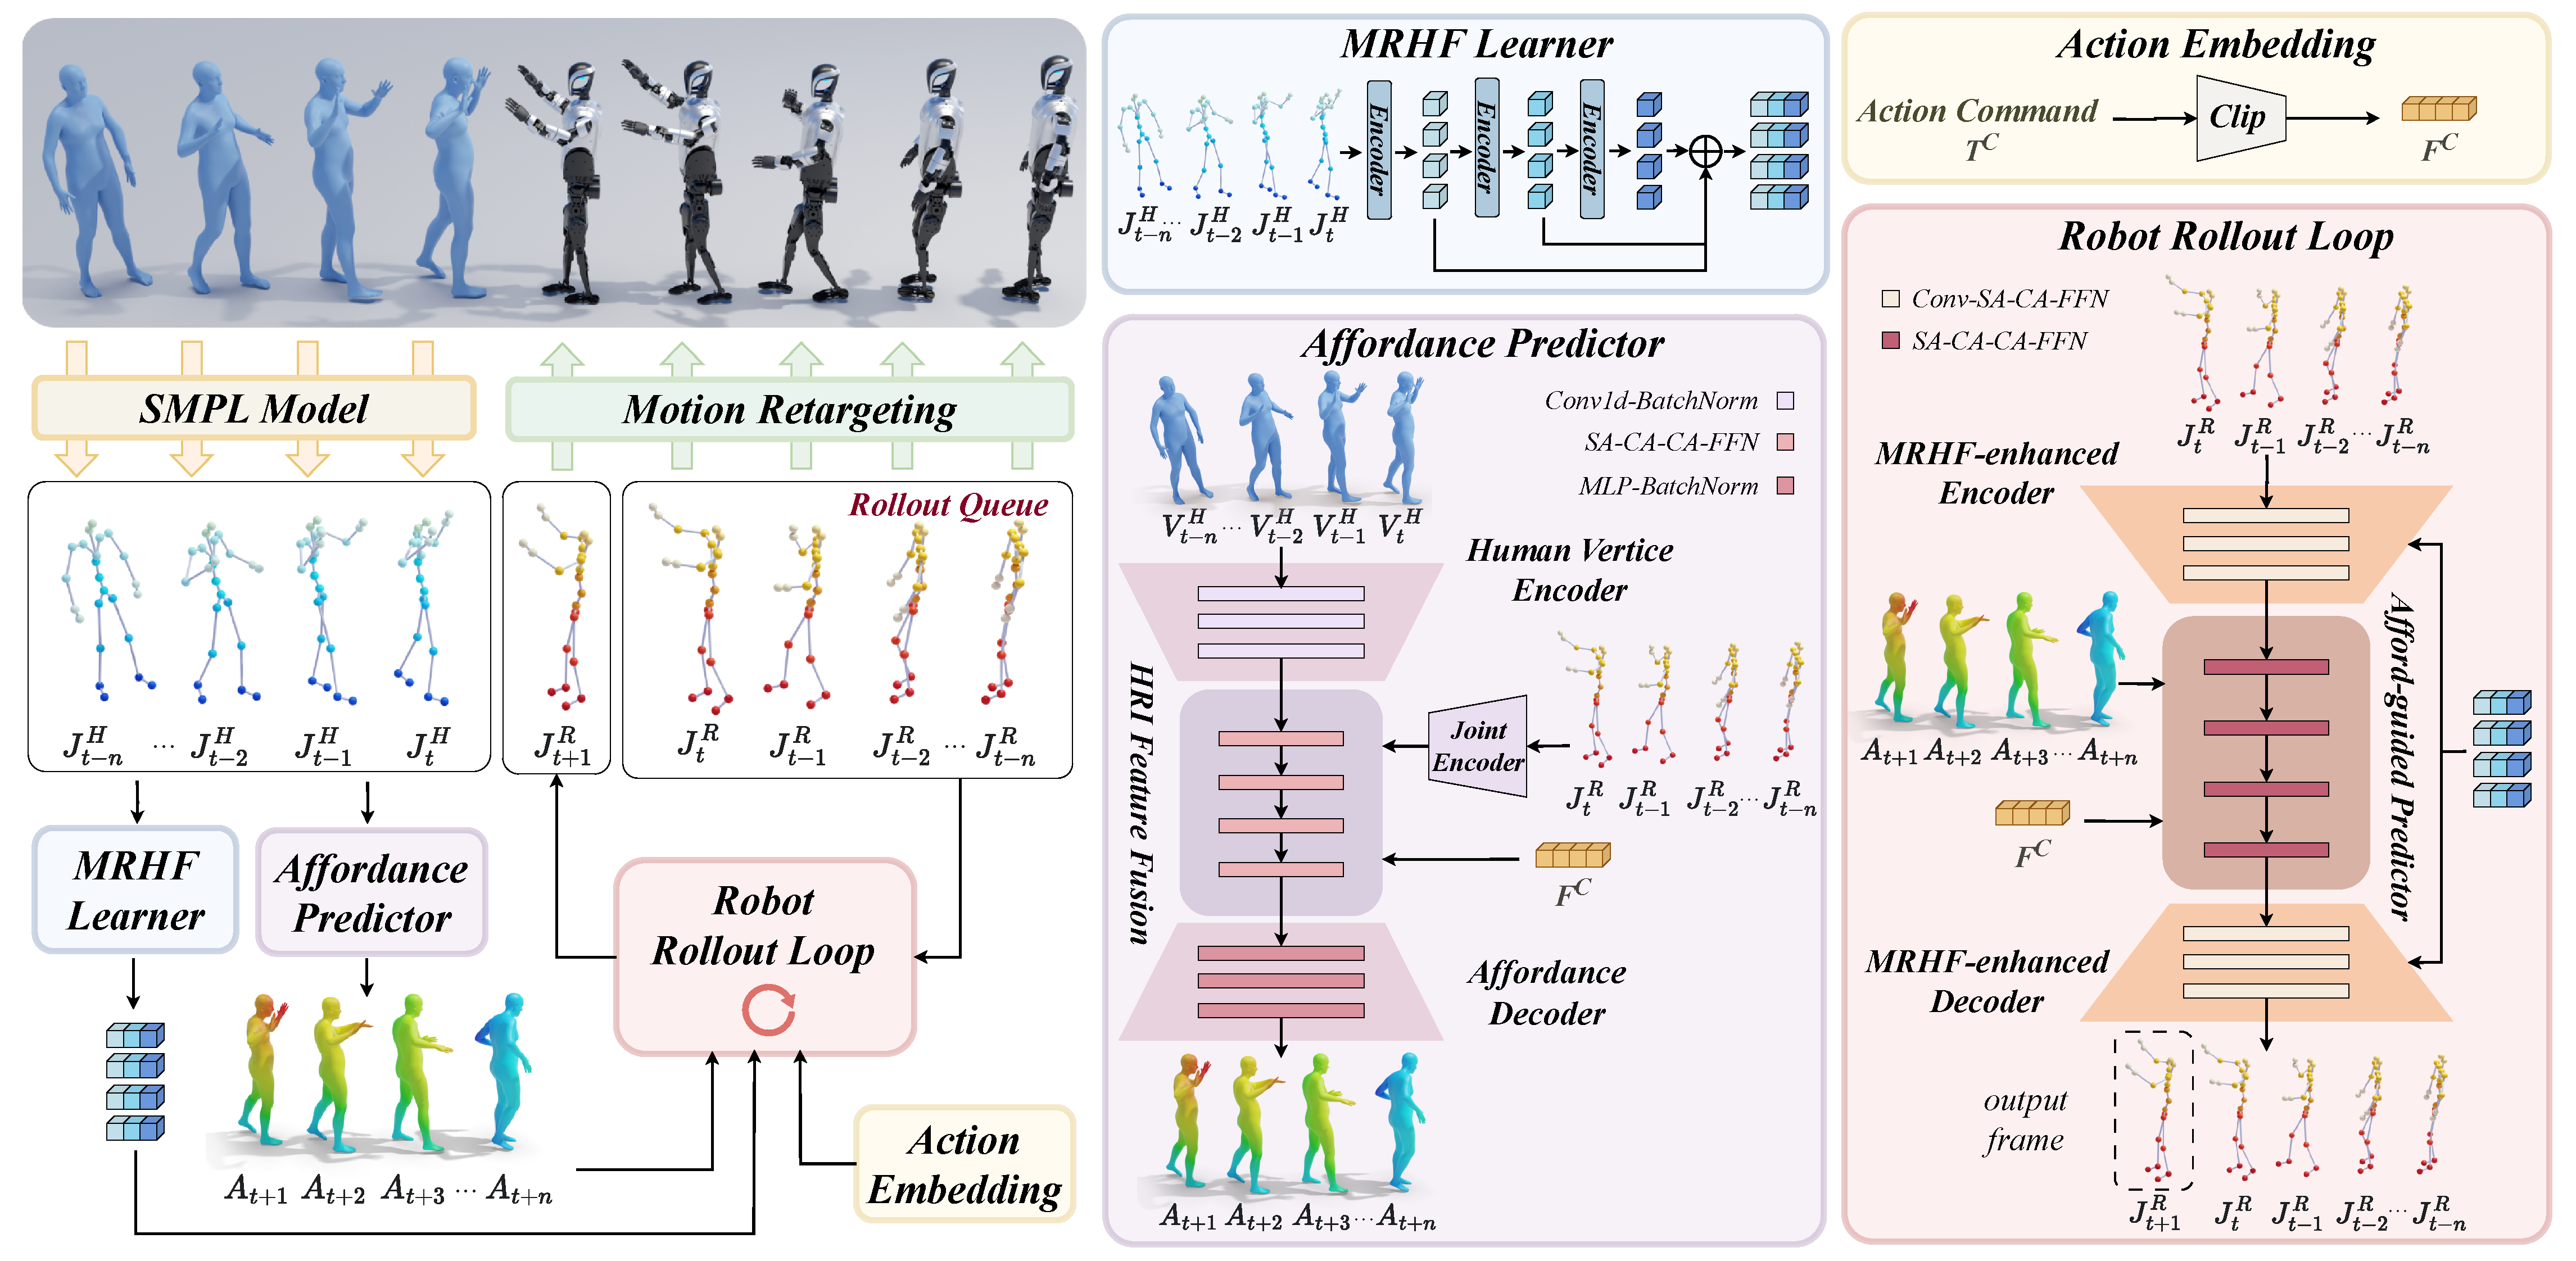
\includegraphics[width=1\linewidth]{images/intermodel-mainv5.pdf}
\vspace{-20pt}
\caption{Overall pipeline of our Robotic Interaction Model. The model ingests text action commands, historical robot joints, observed human joints and SMPL mesh vertices, and processes them through four tightly coupled modules. The Affordance Predictor explicitly estimates dense end-effector–vertex spatial fields to enable dexterous, socially-appropriate contact reasoning; the Multi-Resolution Human Feature (MRHF) Learner fuses hierarchical temporal cues to boost situational awareness; the Robot Rollout Loop leverages these affordance and human features to iteratively generate coherent, context-adaptive joint trajectories for real-time responsiveness; and finally, the Motion Retargeting module maps each predicted skeleton frame to robot-specific angle axis.}
\label{fig:interactiveModel}
\vspace{-10pt}
\end{figure*}
% Real-time, context-aware motion generation remains a challenging problem in human-robot interaction, especially in dynamic and contact-rich scenarios. Prior works~\cite{wang2021multi,xu2024regennet,mueller2024massively} often lack sufficient responsiveness and realistic interaction dynamics.

% To address these challenges, we propose a novel Robotic Interaction Model capable of generating coherent and timely humanoid robot motions for seamless human-robot interactions. Our model is composed of three main modules:

% \begin{itemize}
%     \item \textbf{Affordance Predictor}, which captures fine-grained spatial relationships between robot end-effectors and human body vertices, guiding precise and socially appropriate interactive actions.
%     \item \textbf{Multi-Resolution Human Feature (MRHF) Learner}, which extracts hierarchical temporal features from human motion to enhance situational awareness and response diversity.
%     \item \textbf{Robot Rollout Loop}, which generates robot motions in a frame-by-frame manner to ensure real-time responsiveness and long-term stability.
% \end{itemize}

% \subsection{Model Input and Output}

% Our model generates robot motions online by conditioning on three inputs at each timestep (Fig.~\ref{fig:interactiveModel}): 

% (1) a textual command \(T^C\), representing the intended interaction (e.g., \textit{``High-five''}, \textit{``Handshake''}); 

% (2) historical robot joint skeletons \(J^{R}_{t-n \sim t}\), encoding recent robot motion; 

% (3) observed human motion, including joint skeletons \(J^{H}_{t-n \sim t}\) and SMPL mesh vertices \(V^{H}_{t-n \sim t}\), derived from pose and translation parameters from motion capture (Section ~\ref{sec:mocap}).

% These inputs provide both semantic intent and physical interaction context, enabling the model to predict a short sequence of future robot joint skeletons \(J^{R}_{t+1 \sim t+k}\), because sequence supervision can benefit the consistency of predicted robot motion. However, only the immediate next frame \(J^{R}_{t+1}\) is executed and appended to the rollout queue for the next prediction. This frame-by-frame rollout strategy is crucial for:

% \begin{itemize}
%     \item \textbf{Responsiveness}: adapting to rapid or unexpected changes in human behavior;
%     \item \textbf{Robustness}: mitigating error accumulation common in offline motion generation;
%     \item \textbf{Coherence}: maintaining consistent and fluid robot behavior by conditioning on updated observations each step.
% \end{itemize}

% This mechanism mirrors human interactive behavior, continuously adjusting actions based on perceptual feedback.

% \subsection{Semantic Action Embedding}

% To embed semantic intent, the input command \(T^C\) is encoded into a compact action feature \(F^C\) using a pre-trained CLIP text encoder~\cite{radford2021learning}. This embedding guides downstream modules in generating context-aware motions aligned with the intended interaction.

% \subsection{Affordance Predictor Module}

% Physical and social interactions require precise knowledge of where and how a robot should contact a human. Our Affordance Predictor models a dense spatial affordance field that estimates distances between robot end-effectors (robot hands) and every human body vertex, enabling fine-grained contact reasoning.

% The module encodes the human SMPL mesh sequence \(V^H_{t-n \sim t}\) with a PointNet-based Human Vertice Encoder, generating vertex-wise features \(F^{V^H}_{t-n \sim t}\). These features are fused with the robot’s motion history \(J^R_{t-n \sim t}\) and action embedding \(F^C\) via an encoder-decoder transformer to produce refined interaction features. An MLP-based Affordance Decoder then outputs the dense affordance field \(A_{t+1 \sim t+k}\), informing the robot where to interact in a socially appropriate and physically feasible manner.

% \subsection{MRHF Learner Module}

% Human behavior is temporally hierarchical, with cues evolving at different speeds. To capture this, the MRHF Learner extracts multi-resolution features from the human skeleton sequence \(J^{H}_{t-n \sim t}\) using stacked convolutional and transformer layers. These features encode short-term nuances and long-term behavioral intent, which are concatenated to form the Multi-Resolution Human Feature \(F^{H_{MR}}_{t-n \sim t}\).

% The MRHF enhances the robot's ability to synthesize responses that are temporally coherent and contextually relevant, allowing adaptation to sudden changes while maintaining smooth interaction flow.

% \subsection{Robot Rollout Loop Module}

% To generate natural and responsive robot motions, the Robot Rollout Loop synthesizes actions frame-by-frame, avoiding the error accumulation of offline full-sequence prediction.

% Within this loop, an MRHF-enhanced Encoder processes historical robot motion \(J^{R}_{t-n \sim t}\) together with human features \(F^{H_{MR}}_{t-n \sim t}\) to extract context-aware representations \(F^{R}_{t-n \sim t}\). These are combined with affordance predictions \(A_{t+1 \sim t+k}\) and action embedding \(F^C\) via an Affordance-guided Predictor, yielding spatially aware features \(F^{R'}_{t+1 \sim t+k}\).

% A corresponding MRHF-enhanced Decoder then generates future robot joint sequences \(J^{R}_{t+1 \sim t+k}\). Only the immediate next pose \(J^{R}_{t+1}\) is forwarded to the Motion Retargeting Module for execution and rollout updates.

% This iterative process ensures the robot's motions remain coherent over time while adapting fluidly to evolving human actions.

% \subsection{Robot Motion Retargeting}

% The final predicted joint skeletons are transformed into robot-specific motion parameters using a retargeting module. This module employs a transformer-based spatial encoder capturing inter-joint relationships, followed by a bidirectional GRU that models temporal dynamics. The result is smooth, physically plausible robot motion suitable for execution on the target platform.


% Overall, our Robotic Interaction Model effectively balances real-time responsiveness, motion coherence, and social appropriateness, enabling natural and seamless human-robot interactions in dynamic environments.







